\documentclass{beamer}

\usetheme{Singapore}
\usecolortheme{rose}
\setbeamercovered{transparent}


\usepackage{graphicx}
\usepackage{pgfplots} % tikz
\usepackage{minted} % sudo aptitude install python3-pygments
%\usepackage{amsmath}
%\usepackage{amsthm}
%\usepackage{amssymb}
%\usepackage{amsfonts}
%\usepackage{xcolor}

\title[Introducci\'on a \LaTeX]{Escribiendo ciencia con estilo:\\
  \textbf{Introducci\'on a \LaTeX}}
\subtitle{\textcolor{brown}{\textsc{Escuela de Verano UdeC 2024}}}
\author[RRC]{Ramiro Rebolledo}
\institute[UdeC]{Departamento de Agroindustrias\\
  Facultad de Ingenier\'ia Agr\'icola\\
  Universidad de Concepci\'on}
\subject{\LaTeX}
\date{Sesi\'on 1: Viernes 5 de enero de 2024}%{\today}

\begin{document}

% \begin{frame}[fragile]
%   \begin{minted}[frame=single]{python}
%     >>> type(-12)
%   \end{minted}
% \end{frame}

%   \mint{python}|    >>> 'Hola '+'Mundo'|
% \mintinline{python}{print(x**2)}


\begin{frame}
  \titlepage
\end{frame}

% ------------------------------------------------------------------------------
% ------------------------------------------------------------------------------
% ------------------------------------------------------------------------------
\section{Introducci\'on}
\begin{frame}
  \frametitle{}
  \begin{center}
    \Large\structure{Introducci\'on}
  \end{center}
\end{frame}

% ------------------------------------------------------------------------------

\begin{frame}
  \frametitle{}

  En 1978, \structure{Donald Knuth} dise\~na un sistema de composici\'on
  tipogr\'afica de \structure{bajo nivel} denominado \structure{\TeX}.
  \vspace{20px}
  
  \begin{figure}
    \centering
    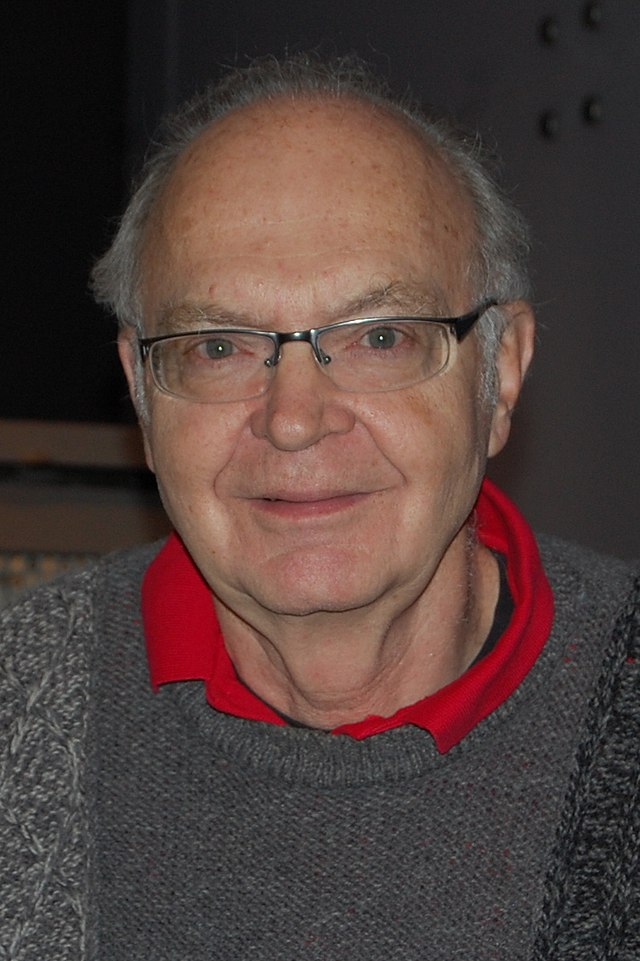
\includegraphics[scale=0.15]{img/Donald_Knuth.jpg}
    % \caption{Donald Knuth}
    
    \structure{Donald Knuth}
    %\label{Donald_Knuth}
  \end{figure}
\end{frame}


% ------------------------------------------------------------------------------

\begin{frame}
  \frametitle{}
  
  \begin{block}{\TeX:}
    \begin{itemize}
    \item Es muy potente, pero su sintaxis puede ser compleja y no amigable para
      los usuarios no expertos.
      \pause
    \item Permite un control detallado sobre el diseño tipogr\'afico
      y la composici\'on del documento.
      Es especialmente adecuado para expertos que desean un control fino sobre
      cada aspecto del dise\~no.
      \pause
    \item No es un procesador de textos, sino un conjunto de macros y un
      lenguaje de programaci\'on.
    \end{itemize}
  \end{block}
\end{frame}

% ------------------------------------------------------------------------------

\begin{frame}
  \frametitle{}
  
  \begin{block}{?`Qu\'e es \LaTeX?}
    \begin{itemize}
    \item \structure{\LaTeX}, escrito por \structure{Leslie Lamport} en 1984,
      est\'a formado por un gran conjunto de macros de \TeX\, con la intenci\'on
      de facilitar el uso de \TeX.
    \end{itemize}
  \end{block}
  
  \vspace{-10px}
  
  \begin{figure}
    \centering
    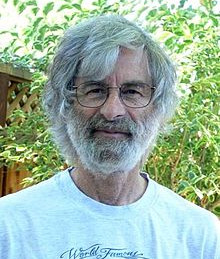
\includegraphics[scale=0.6]{img/Leslie_Lamport.jpg}
    % \caption{Leslie Lamport}
    
    \structure{Leslie Lamport}
    %\label{Leslie_Lamport}
  \end{figure}

  \pause

  \vspace{-15px}

  \begin{alertblock}{}
    \hspace{60px}
    \structure{\LaTeX}
    \hspace{10px}=\hspace{10px}
    \TeX+\LaTeX+mejoras posteriores.
  \end{alertblock}

\end{frame}

% ------------------------------------------------------------------------------

\begin{frame}[fragile]
  \frametitle{Caracter\'isticas clave de \LaTeX}

  \begin{enumerate}
  \item \textbf{Transportabilidad:}
    Los ficheros \mintinline{latex}{.tex} s\'olo contienen
    \structure{texto plano}, por lo que son peque\~nos, portables
    y manipulables en cualquier plataforma.
    \pause
  \item \textbf{Sistematizaci\'on:}
    \LaTeX\, Maneja el formato del documento, evitando preocupaciones sobre
    saltos de p\'agina, justificaciones, referencias cruzadas,
    \'indices, \alert{bibliograf\'ia}, etc.
    \pause
  \item \textbf{Versatilidad:}
    Esencialmente, puede hacer cualquier cosa, limitada s\'olo por la
    imaginaci\'on del usuario.
    \pause
  \item \textbf{Flexibilidad:}
    Permite la creaci\'on y modificaci\'on de comandos y
    entornos, facilitando la escritura de documentos.
    \pause
  \item \textbf{Actualizaci\'on:}
    \LaTeX\, es mejorado continuamente a trav\'es de contribuciones altruistas,
    con paquetes compartidos como \structure{software libre}.
  \end{enumerate}

\end{frame}

% ------------------------------------------------------------------------------

% ------------------------------------------------------------------------------
% ------------------------------------------------------------------------------
% ------------------------------------------------------------------------------
\section{Ventajas e inconvenientes}
\begin{frame}
  \frametitle{}
  \begin{center}
    \Large\structure{Ventajas e inconvenientes}
  \end{center}
\end{frame}

% ------------------------------------------------------------------------------

\begin{frame}
  \frametitle{}
  \begin{columns}[T]
    \begin{column}{0.48\textwidth}
      \begin{block}{Ventajas}
        \begin{itemize}
        \item Composici\'on de f\'ormulas f\'acil, r\'apido, y con
          la m\'as alta calidad tipogr\'afica
          \pause
        \item Gesti\'on f\'acil de bibliograf\'ia,
          referencias cruzadas, etc.
          \pause
        \item Independiente de la plataforma: Linux, Windows, OSX,\dots
          \pause
        \item \structure{Software libre}
          (muchos paquetes adicionales)
          \pause
        \item Salida postscript, PDF,\dots
          \pause
        \item Separación de contenido y formato (puede ser desventaja)
        \end{itemize}
      \end{block}
    \end{column}
    \pause
    \hfill

    \begin{column}{0.48\textwidth}
      \begin{block}{}
        \begin{itemize}
        \item \alert{Retrocompatibilidad}
        \end{itemize}
      \end{block}

      \pause
      \begin{alertblock}{Inconvenientes}
        \begin{itemize}
        \item La curva de aprendizaje es m\'as pronunciada
          \pause
        \item Dise\~nar un nuevo documento puede ser dif\'icil si las plantillas
          predefinidas no se ajustan a nuestras necesidades
          \pause
        \item La detecci\'on y manejo de errores pueden ser m\'as compleja
      \end{itemize}
      \end{alertblock}
    \end{column}
  \end{columns}
\end{frame}

\begin{frame}
  \frametitle{Curva de aprendizaje de \LaTeX}

  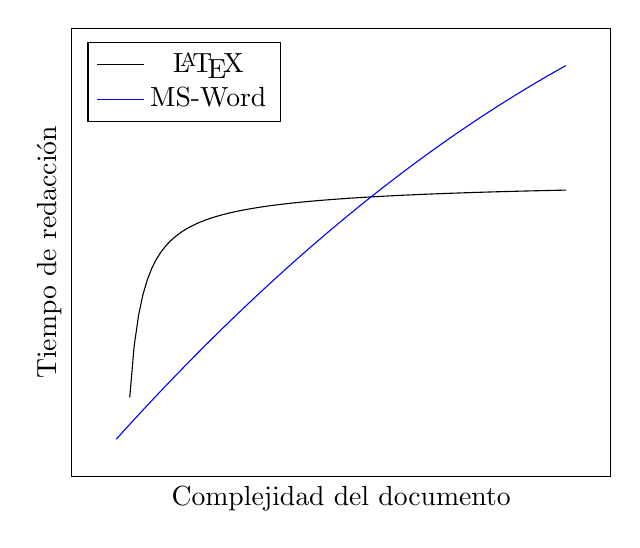
\begin{tikzpicture}
    \begin{axis}[
      xlabel={Complejidad del documento},
      ylabel={Tiempo de redacci\'on},
      legend pos=north west,
      xtick=\empty,
      ytick=\empty,
      grid=both,
      ]

      \addplot[black, domain=0.03:1, samples=100] {(x^3-1)/(x^3+x)+40};
      \addplot[blue, domain=0:1, samples=100] {-20*(x-2)^2+80};
      
      \legend{\LaTeX, MS-Word}
    \end{axis}
  \end{tikzpicture}
  
\end{frame}

% ------------------------------------------------------------------------------
% ------------------------------------------------------------------------------
% ------------------------------------------------------------------------------
% ------------------------------------------------------------------------------
\section{Usos de \LaTeX}
\begin{frame}
  \frametitle{}
  \begin{center}
    \Large\structure{Usos de \LaTeX}
  \end{center}
\end{frame}

% ------------------------------------------------------------------------------

\begin{frame}
  \frametitle{Usos de \LaTeX}


  \begin{itemize}
  \item Libros y apuntes
    \pause
  \item Presentaciones
    \pause
  \item Art\'iculos
    \pause
  \item Cert\'amenes y lista de ejercicios
    \pause
  \item Cartas e informes
    \pause
  \item Posters
    \pause
  \item Su sintaxis (o similar) se utiliza en muchos software, como
    matlab, geogebra, LMS Canvas, notebooks jupyter de python, etc.
  \end{itemize}
\end{frame}

% ------------------------------------------------------------------------------
% ------------------------------------------------------------------------------
% ------------------------------------------------------------------------------
\section{Manos a la obra}
\begin{frame}
  \frametitle{}
  \begin{center}
    \Large\structure{Manos a la obra}
  \end{center}
\end{frame}

% ------------------------------------------------------------------------------

\begin{frame}
  \frametitle{}

  Para comenzar este taller:
  \vspace{10px}
  
  \begin{itemize}
  \item Ingresa a \url{https://es.overleaf.com}
  \item Crea una cuenta (bot\'on Register)
  \end{itemize}
  \vspace{10px}
  
  \begin{figure}
    \centering
    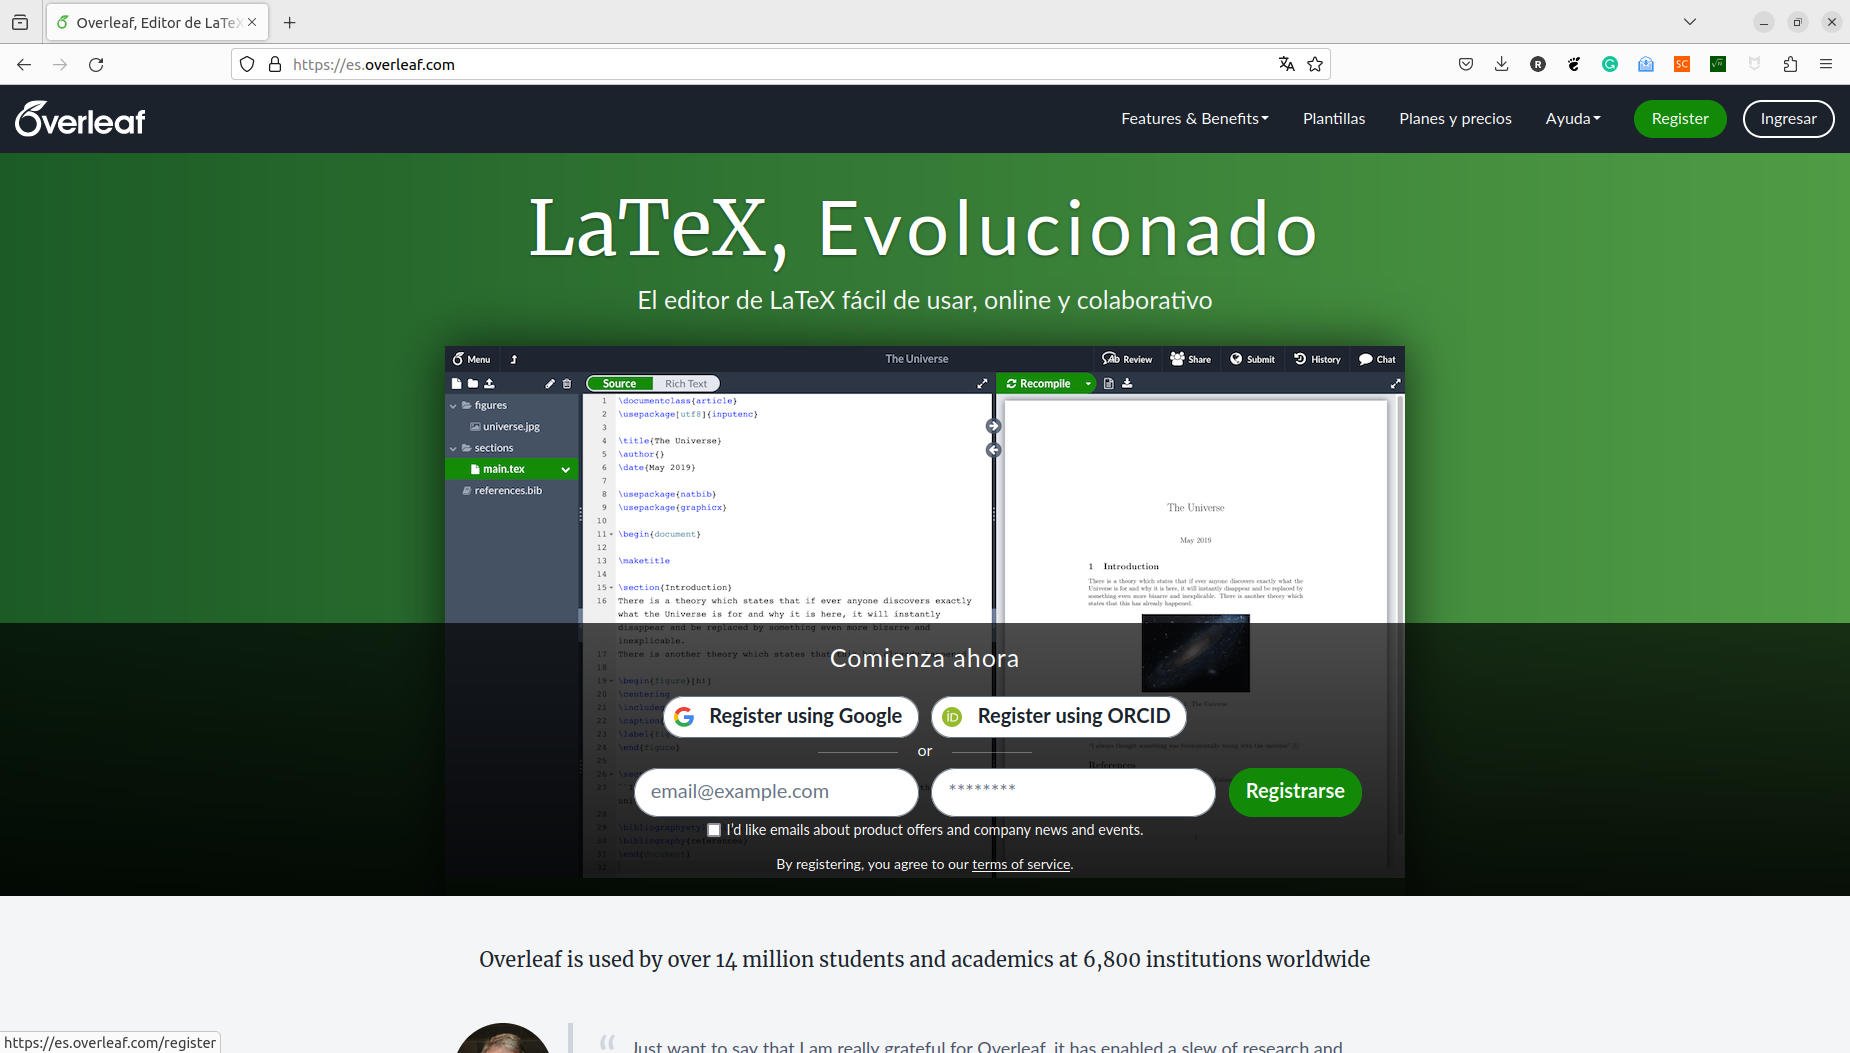
\includegraphics[scale=0.17]{img/overleaf.png}
  \end{figure}

\end{frame}

% ------------------------------------------------------------------------------

\begin{frame}

  Enlaces \'utiles
  \vspace{10px}
  

  \begin{itemize}
  \item Lista de s\'imbolos y tutoriales:
    \begin{itemize}
    \item \url{https://manualdelatex.com/simbolos}
    \item \url{https://manualdelatex.com/tutoriales}
    \end{itemize}
  \item https://detexify.kirelabs.org
  \item Y comencemos
  \end{itemize}
  
\end{frame}


\end{document}
